\documentclass[12pt,a4paper]{article}

% ============================================================
% PACKAGES
% ============================================================

\usepackage[utf8]{inputenc}
\usepackage[T1]{fontenc}
\usepackage{lmodern}
\usepackage{tikz}
\usetikzlibrary{positioning}

\usepackage[english]{babel}

\usepackage{geometry}
\geometry{
    left=2.5cm,
    right=2.5cm,
    top=2.5cm,
    bottom=2.5cm
}

\usepackage{graphicx}
\usepackage{xcolor}
\usepackage{hyperref}
\usepackage{booktabs}
\usepackage{longtable}
\usepackage{array}
\usepackage{enumitem}
\usepackage{listings}
\usepackage{float}
\usepackage{fancyhdr}
\usepackage{titlesec}
\usepackage{caption}
\usepackage{tikz}
\usepackage{amsmath}

% ============================================================
% HYPERLINK CONFIGURATION
% ============================================================

\hypersetup{
    colorlinks=true,
    linkcolor=blue,
    urlcolor=blue,
    citecolor=blue,
    pdftitle={Developer Manual - Football Tournament Management System},
    pdfauthor={Rostand Cedrix Assonfo Demaboi}
}

% ============================================================
% CODE LISTING CONFIGURATION
% ============================================================

\definecolor{codegray}{gray}{0.95}
\definecolor{codecomment}{gray}{0.45}

\lstset{
    backgroundcolor=\color{codegray},
    basicstyle=\ttfamily\small,
    breaklines=true,
    frame=single,
    numbers=left,
    numberstyle=\tiny,
    keywordstyle=\bfseries,
    commentstyle=\itshape\color{codecomment},
    showstringspaces=false,
    tabsize=4
}

% ============================================================
% HEADER / FOOTER
% ============================================================

\pagestyle{fancy}
\fancyhf{}

\lhead{Football Tournament Management System}
\rhead{Developer Manual}
\cfoot{\thepage}

% ============================================================
% DOCUMENT
% ============================================================

\begin{document}

% ============================================================
% TITLE PAGE
% ============================================================

\begin{titlepage}

\centering

\vspace*{2cm}

{\Huge \textbf{Football Tournament Management System}\par}

\vspace{1cm}

{\LARGE Developer Manual\par}

\vspace{2cm}

{\large
Technical Documentation for Developers
\par}

\vspace{1.5cm}

\begin{tabular}{ll}
\textbf{Author:} & Rostand Cedrix Assonfo Demaboi \\
\textbf{Institution:} & Technische Hochschule Georg Agricola, Bochum \\
\textbf{Module:} & Introduction to Database Management Systems \\
\textbf{Semester:} & Summer Term 2026 \\
\end{tabular}

\vfill

{\large Version 1.0}

\vspace{0.5cm}

{\large \today}

\end{titlepage}

% ============================================================
% TABLE OF CONTENTS
% ============================================================

\tableofcontents
\newpage

% ============================================================
% 1. INTRODUCTION
% ============================================================

\section{Introduction}

\subsection{Purpose of this Document}

This document is the technical developer manual for the
Football Tournament Management System.

Its purpose is to provide future developers with the information
required to understand, install, maintain, test, and extend the
application.

Unlike the user manual, which focuses on how to use the application,
this document focuses on the internal architecture, source code,
database structure, API, business logic, and development workflow.

\subsection{System Overview}

The Football Tournament Management System is an application designed
to organize, track, and administer football competitions.

The system supports the management of:

\begin{itemize}
    \item tournaments,
    \item teams,
    \item matches,
    \item match scores,
    \item referees,
    \item tournament standings.
\end{itemize}

The application follows a decoupled architecture composed of a
backend REST API, a graphical frontend, and a relational database.

\subsection{User Roles}

The system provides two main user roles.

\subsubsection{Organizer Mode}

Organizer Mode provides write access to the system.

An authenticated organizer can:

\begin{itemize}
    \item create tournaments,
    \item modify tournaments,
    \item delete tournaments,
    \item create teams,
    \item modify teams,
    \item delete teams,
    \item schedule matches,
    \item update match scores,
    \item delete matches.
\end{itemize}

Authentication is performed using an API key transmitted through
the \texttt{X-API-Key} HTTP header.

\subsubsection{Viewer Mode}

Viewer Mode is a read-only mode.

A viewer can:

\begin{itemize}
    \item view tournaments,
    \item view teams,
    \item view matches,
    \item view match scores,
    \item view tournament standings.
\end{itemize}

% ============================================================
% 2. TECHNOLOGY STACK
% ============================================================

\section{Technology Stack}

\begin{table}[H]
\centering
\begin{tabular}{ll}
\toprule
\textbf{Component} & \textbf{Technology} \\
\midrule
Backend & Python / FastAPI \\
Frontend & Python / Tkinter \\
Database & Relational SQL Database \\
Communication & REST API \\
Authentication & X-API-Key \\
Containerization & Docker / Docker Compose \\
\bottomrule
\end{tabular}
\caption{Technology stack}
\end{table}

\subsection{Backend}

The backend is implemented as a REST API using FastAPI.

Its responsibilities include:

\begin{itemize}
    \item receiving HTTP requests,
    \item validating input data,
    \item applying business rules,
    \item communicating with the database,
    \item returning HTTP responses.
\end{itemize}

\subsection{Frontend}

The frontend is implemented using Python Tkinter.

It provides a graphical interface for:

\begin{itemize}
    \item viewing tournaments,
    \item viewing teams,
    \item viewing matches,
    \item viewing standings,
    \item performing administrative operations.
\end{itemize}

\subsection{Docker}

Docker Compose is used to orchestrate the application services.

The goal is to provide a reproducible and portable runtime environment.

% ============================================================
% 3. SYSTEM ARCHITECTURE
% ============================================================

\section{System Architecture}

\subsection{Architecture Overview}

The application follows a client-server architecture.

\begin{figure}[H]
\centering

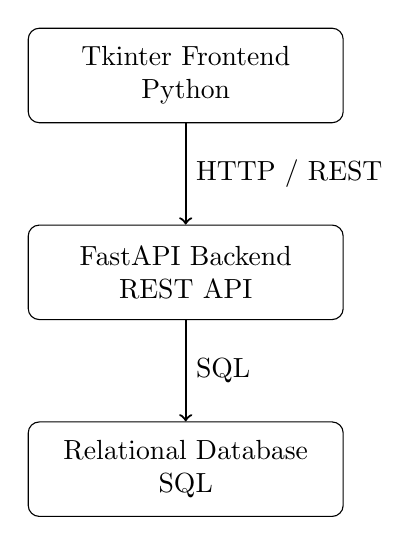
\begin{tikzpicture}[
    node distance=2.5cm,
    box/.style={
        rectangle,
        draw,
        rounded corners,
        minimum width=4cm,
        minimum height=1.2cm,
        align=center
    },
    arrow/.style={
        ->,
        thick
    }
]

\node[box] (frontend)
{Tkinter Frontend\\Python};

\node[box, below of=frontend] (api)
{FastAPI Backend\\REST API};

\node[box, below of=api] (database)
{Relational Database\\SQL};

\draw[arrow] (frontend) -- node[right] {HTTP / REST} (api);
\draw[arrow] (api) -- node[right] {SQL} (database);

\end{tikzpicture}

\caption{System architecture}
\label{fig:architecture}

\end{figure}

\subsection{Frontend Layer}

The frontend is responsible for user interaction.

It communicates with the backend exclusively through the REST API.

The frontend should not directly access the database.

\subsection{Backend Layer}

The backend acts as the central application layer.

It is responsible for:

\begin{itemize}
    \item API endpoints,
    \item authentication,
    \item validation,
    \item business logic,
    \item database access.
\end{itemize}

\subsection{Database Layer}

The database stores persistent application data.

The database is responsible for maintaining:

\begin{itemize}
    \item primary key constraints,
    \item foreign key constraints,
    \item uniqueness constraints,
    \item referential integrity.
\end{itemize}

% ============================================================
% 4. PROJECT STRUCTURE
% ============================================================

\section{Project Structure}

The following structure represents the recommended organization of
the project.

\begin{lstlisting}
football-tournament-manager/
|
+-- backend/
|   +-- ...
|
+-- frontend/
|   +-- football_tournament/
|       +-- ...
|
+-- database/
|   +-- ...
|
+-- tests/
|   +-- ...
|
+-- docker-compose.yml
+-- Dockerfile
+-- requirements.txt
+-- README.md
+-- DEVELOPER_MANUAL.tex
\end{lstlisting}

\subsection{Backend Directory}

The backend directory contains the FastAPI application and all
backend-related components.

\textbf{TODO:} Document the actual backend directories and files
according to the source code.

\subsection{Frontend Directory}

The frontend directory contains the Tkinter graphical application.

\textbf{TODO:} Document the actual frontend modules and their
responsibilities.

\subsection{Tests Directory}

The tests directory contains automated tests.

\textbf{TODO:} Document the actual test structure.

% ============================================================
% 5. INSTALLATION
% ============================================================

\section{Installation and Setup}

\subsection{Prerequisites}

The following software is required:

\begin{itemize}
    \item Git,
    \item Docker,
    \item Docker Compose,
    \item Python 3,
    \item a SQL-compatible database environment.
\end{itemize}

\textbf{TODO:} Specify the exact supported versions.

\subsection{Clone the Repository}

\begin{lstlisting}[language=bash]
git clone <repository-url>
cd football-tournament-manager
\end{lstlisting}

\subsection{Backend Installation}

\textbf{TODO:} Document the exact Python environment and dependency
installation process.

Example:

\begin{lstlisting}[language=bash]
python3 -m venv venv
source venv/bin/activate
pip install -r requirements.txt
\end{lstlisting}

\subsection{Frontend Installation}

The frontend uses a Python virtual environment.

Example:

\begin{lstlisting}[language=bash]
cd frontend
source venv/bin/activate
\end{lstlisting}

% ============================================================
% 6. DOCKER
% ============================================================

\section{Docker and Deployment}

\subsection{Starting the Services}

The complete backend environment can be started using:

\begin{lstlisting}[language=bash]
docker compose up --build -d
\end{lstlisting}

\subsection{Checking Running Containers}

\begin{lstlisting}[language=bash]
docker compose ps
\end{lstlisting}

\subsection{Viewing Logs}

\begin{lstlisting}[language=bash]
docker compose logs
\end{lstlisting}

To inspect a specific service:

\begin{lstlisting}[language=bash]
docker compose logs <service-name>
\end{lstlisting}

\subsection{Stopping the Services}

\begin{lstlisting}[language=bash]
docker compose down
\end{lstlisting}

\textbf{TODO:} Document the exact Docker services defined in
\texttt{docker-compose.yml}.

% ============================================================
% 7. DATABASE DESIGN
% ============================================================

\section{Database Design}

\subsection{Database Overview}

The application uses a relational database to persist tournament,
team, and match information[cite: 1, 2].

\subsection{Entity Relationship Model}

\begin{figure}[H]
\centering

\begin{tikzpicture}[
    entity/.style={
        rectangle,
        draw,
        minimum width=4cm,
        minimum height=1cm,
        align=center
    }
]

\node[entity] (tournament)
{TOURNAMENT};

\node[entity, below left=2.5cm and 2cm of tournament] (team)
{TEAM};

\node[entity, below right=2.5cm and 2cm of tournament] (match)
{MATCH};

\draw[-, thick] (tournament) -- node[left] {1:N} (match);
\draw[-, thick] (team) -- node[below] {participates} (match);

\end{tikzpicture}

\caption{Simplified entity relationship model}
\label{fig:erd}

\end{figure}

\textbf{TODO:} Replace this simplified diagram with the exact
database schema.

% ------------------------------------------------------------
% Tournament
% ------------------------------------------------------------

\subsection{Tournament Table}

\begin{longtable}{llll}
\toprule
\textbf{Column} & \textbf{Type} & \textbf{Constraint} & \textbf{Description}\\
\midrule
id & --- & Primary Key & Unique tournament identifier\\
name & --- & --- & Tournament name\\
start\_date & --- & --- & Tournament start date\\
end\_date & --- & --- & Tournament end date\\
status & --- & --- & Tournament status\\
\bottomrule
\end{longtable}

\textbf{TODO:} Replace types and fields with the actual SQL schema.

% ------------------------------------------------------------
% Team
% ------------------------------------------------------------

\subsection{Team Table}

\begin{longtable}{llll}
\toprule
\textbf{Column} & \textbf{Type} & \textbf{Constraint} & \textbf{Description}\\
\midrule
id & --- & Primary Key & Unique team identifier\\
name & --- & --- & Official team name\\
coach & --- & --- & Coach or manager\\
\bottomrule
\end{longtable}

% ------------------------------------------------------------
% Team / Tournament Association (N:M)
% ------------------------------------------------------------

\subsection{Team/Tournament Association}

The many-to-many ($N:M$) relationship between teams and tournaments is implemented using the \texttt{team\_tournaments} associative entity, ensuring that a team can participate in multiple tournaments and a tournament can include multiple teams[cite: 1, 2].

\begin{itemize}
    \item \textbf{Table Name:} \texttt{team\_tournaments} (or \texttt{TeamTournament})[cite: 1, 2]
    \item \textbf{Composite Primary Key:} (\texttt{team\_id}, \texttt{tournament\_id})[cite: 1, 2]
    \item \textbf{Foreign Keys:} 
    \begin{itemize}
        \item \texttt{team\_id} references \texttt{teams(team\_id)}[cite: 1, 2]
        \item \texttt{tournament\_id} references \texttt{tournaments(tournament\_id)}[cite: 1, 2]
    \end{itemize}
    \item \textbf{Business Purpose:} Prevents duplicate team registrations in the same tournament while maintaining clean referential integrity upon deletion[cite: 1, 2].
\end{itemize}

% ------------------------------------------------------------
% Match
% ------------------------------------------------------------

\subsection{Match Table}

\begin{longtable}{llll}
\toprule
\textbf{Column} & \textbf{Type} & \textbf{Constraint} & \textbf{Description}\\
\midrule
id & --- & Primary Key & Unique match identifier\\
tournament\_id & --- & Foreign Key & Related tournament\\
home\_team\_id & --- & Foreign Key & Home team\\
away\_team\_id & --- & Foreign Key & Away team\\
date & --- & --- & Match date\\
home\_score & --- & --- & Home team score\\
away\_score & --- & --- & Away team score\\
referee & --- & --- & Assigned referee\\
\bottomrule
\end{longtable}

% ============================================================
% 8. REST API
% ============================================================

\section{REST API}

\subsection{API Base URL}

The default development API URL is:

\begin{lstlisting}
http://localhost:8000
\end{lstlisting}

\subsection{Authentication}

Administrative operations require the HTTP header:

\begin{lstlisting}
X-API-Key: <API-KEY>
\end{lstlisting}

Example:

\begin{lstlisting}[language=bash]
curl -X POST http://localhost:8000/tournaments \
     -H "X-API-Key: mykey"
\end{lstlisting}

\subsection{Tournament Endpoints}

\begin{longtable}{lll}
\toprule
\textbf{Method} & \textbf{Endpoint} & \textbf{Description}\\
\midrule
GET & /tournaments & List tournaments\\
POST & /tournaments & Create tournament\\
PUT & /tournaments/\{id\} & Update tournament\\
DELETE & /tournaments/\{id\} & Delete tournament\\
\bottomrule
\end{longtable}

\textbf{TODO:} Replace these endpoints with the exact endpoints
implemented by the backend.

\subsection{Team Endpoints}

\begin{longtable}{lll}
\toprule
\textbf{Method} & \textbf{Endpoint} & \textbf{Description}\\
\midrule
GET & /teams & List teams\\
POST & /teams & Create team\\
PUT & /teams/\{id\} & Update team\\
DELETE & /teams/\{id\} & Delete team\\
\bottomrule
\end{longtable}

\subsection{Match Endpoints}

\begin{longtable}{lll}
\toprule
\textbf{Method} & \textbf{Endpoint} & \textbf{Description}\\
\midrule
GET & /matches & List matches\\
POST & /matches & Create match\\
PUT & /matches/\{id\} & Update match\\
DELETE & /matches/\{id\} & Delete match\\
\bottomrule
\end{longtable}

% ============================================================
% 9. BACKEND ARCHITECTURE
% ============================================================

\section{Backend Architecture}

\subsection{Request Processing}

A typical API request follows this sequence:

\begin{enumerate}
    \item The frontend sends an HTTP request.
    \item FastAPI receives the request.
    \item Authentication is checked when required.
    \item Input data is validated.
    \item Business logic is executed.
    \item The database is queried or modified.
    \item The backend returns an HTTP response.
    \item The frontend updates its display.
\end{enumerate}

\subsection{API Routers}

\textbf{TODO:} Document the actual FastAPI routers implemented in
the source code.

Example:

\begin{lstlisting}[language=python]
@router.get("/tournaments")
def get_tournaments():
    ...
\end{lstlisting}

\subsection{Data Validation}

\textbf{TODO:} Document the Pydantic schemas and validation rules.

% ============================================================
% 10. FRONTEND ARCHITECTURE
% ============================================================

\section{Frontend Architecture}

\subsection{Main Interface}

The graphical interface is organized around several tabs:

\begin{itemize}
    \item Tournaments,
    \item Teams,
    \item Matches,
    \item Standings.
\end{itemize}

\subsection{Connection Panel}

At startup, the frontend requests:

\begin{itemize}
    \item API URL,
    \item optional X-API-Key.
\end{itemize}

Leaving the API key empty provides Viewer Mode.

Providing a valid administrative key enables Organizer Mode.

\subsection{Tournament Tab}

The Tournament tab displays the registered competitions.

\subsection{Teams Tab}

The Teams tab displays participating clubs and their information.

\subsection{Matches Tab}

The Matches tab provides access to fixtures and scores.

A tournament selector allows filtering matches by tournament.

\subsection{Standings Tab}

The Standings tab dynamically calculates tournament rankings.

% ============================================================
% 11. BUSINESS LOGIC
% ============================================================

\section{Business Logic}

\subsection{Match Management}

A match is associated with:

\begin{itemize}
    \item one tournament,
    \item one home team,
    \item one away team,
    \item a date,
    \item optionally a score,
    \item a referee.
\end{itemize}

\subsection{Score Management}

Scores can be updated by an authenticated organizer.

\subsection{Standings Calculation}

The standings are calculated from the results of matches.

The ranking contains at least:

\begin{itemize}
    \item points,
    \item wins,
    \item draws,
    \item losses,
    \item goals scored,
    \item goals conceded,
    \item goal difference.
\end{itemize}

\textbf{TODO:} Document the exact ranking and tie-breaking algorithm.

For example:

\[
\text{Goal Difference}
=
\text{Goals For}
-
\text{Goals Against}
\]

\textbf{TODO:} Specify the exact points system implemented by the
application.

% ============================================================
% 12. AUTHENTICATION
% ============================================================

\section{Authentication and Authorization}

\subsection{API Key}

The API uses an API key mechanism based on the HTTP
\texttt{X-API-Key} header.

\subsection{Viewer Permissions}

Viewer users have read-only access.

\subsection{Organizer Permissions}

Organizer users have read and write access.

\begin{table}[H]
\centering
\begin{tabular}{lcc}
\toprule
\textbf{Operation} & \textbf{Viewer} & \textbf{Organizer}\\
\midrule
Read tournaments & Yes & Yes\\
Read teams & Yes & Yes\\
Read matches & Yes & Yes\\
Read standings & Yes & Yes\\
Create data & No & Yes\\
Update data & No & Yes\\
Delete data & No & Yes\\
\bottomrule
\end{tabular}
\caption{Authorization matrix}
\end{table}

% ============================================================
% 13. ERROR HANDLING
% ============================================================

\section{Error Handling}

The API should provide meaningful HTTP status codes.

\begin{table}[H]
\centering
\begin{tabular}{cl}
\toprule
\textbf{Status} & \textbf{Meaning}\\
\midrule
200 & Successful request\\
201 & Resource successfully created\\
400 & Invalid request\\
401 & Unauthorized\\
404 & Resource not found\\
409 & Database or resource conflict\\
500 & Internal server error\\
\bottomrule
\end{tabular}
\caption{HTTP error codes}
\end{table}

\textbf{TODO:} Verify the exact status codes implemented by the API.

% ============================================================
% 14. DATABASE INTEGRITY
% ============================================================

\section{Database Integrity}

Database operations must preserve referential integrity.

Examples include:

\begin{itemize}
    \item a match must reference an existing tournament,
    \item a match must reference existing teams,
    \item referenced entities should not be deleted if this would
    violate database constraints.
\end{itemize}

The application respects database referential integrity constraints
when deleting obsolete teams or matches.

\textbf{TODO:} Document the exact foreign-key and ON DELETE rules.

% ============================================================
% 15. TESTING
% ============================================================

\section{Testing}

\subsection{Testing Strategy}

The project should test the following layers:

\begin{itemize}
    \item database,
    \item business logic,
    \item REST API,
    \item frontend.
\end{itemize}

\subsection{Unit Tests}

Unit tests should validate isolated business rules.

Example:

\begin{lstlisting}[language=python]
def test_goal_difference():
    assert calculate_goal_difference(3, 1) == 2
\end{lstlisting}

\subsection{API Tests}

API tests should verify:

\begin{itemize}
    \item successful requests,
    \item invalid requests,
    \item authentication,
    \item missing resources,
    \item database conflicts.
\end{itemize}

\subsection{Database Tests}

Database tests should verify:

\begin{itemize}
    \item primary keys,
    \item foreign keys,
    \item uniqueness,
    \item deletion constraints.
\end{itemize}

% ============================================================
% 16. DEVELOPMENT WORKFLOW
% ============================================================

\section{Development Workflow}

A recommended development workflow is:

\begin{enumerate}
    \item Pull the latest version of the repository.
    \item Create a dedicated feature branch.
    \item Implement the change.
    \item Run automated tests.
    \item Test the API.
    \item Test the frontend.
    \item Verify database integrity.
    \item Update the documentation.
    \item Commit the changes.
    \item Create a pull request.
\end{enumerate}

Example:

\begin{lstlisting}[language=bash]
git checkout -b feature/new-functionality

# Implement changes

git add .
git commit -m "Add new functionality"

git push origin feature/new-functionality
\end{lstlisting}

% ============================================================
% 17. TROUBLESHOOTING
% ============================================================

\section{Troubleshooting}

\subsection{Backend Does Not Start}

Check the Docker services:

\begin{lstlisting}[language=bash]
docker compose ps
\end{lstlisting}

Then inspect the logs:

\begin{lstlisting}[language=bash]
docker compose logs
\end{lstlisting}

\subsection{Frontend Cannot Connect}

Verify that the API is running on:

\begin{lstlisting}
http://localhost:8000
\end{lstlisting}

Also verify the API URL entered in the connection dialog.

\subsection{Organizer Mode Does Not Work}

Check that the correct API key is provided through the
\texttt{X-API-Key} field.

\textbf{TODO:} Document how the API key is configured in the
actual application.

% ============================================================
% 18. MAINTENANCE
% ============================================================

\section{Maintenance}

\subsection{Dependency Updates}

Document how Python dependencies are updated.

Example:

\begin{lstlisting}[language=bash]
pip install --upgrade <package>
pip freeze > requirements.txt
\end{lstlisting}

\subsection{Database Changes}

Database schema changes should be documented and tested before
being deployed.

\textbf{TODO:} Document whether the project uses SQL migration tools
such as Alembic or another migration mechanism.

\subsection{Logging}

\textbf{TODO:} Document the application's logging system and
log locations.

% ============================================================
% 19. EXTENDING THE APPLICATION
% ============================================================

\section{Extending the Application}

Future developers may extend the application with additional
functionality.

Potential extensions include:

\begin{itemize}
    \item player management,
    \item yellow and red cards,
    \item stadium management,
    \item player statistics,
    \item tournament groups,
    \item notifications,
    \item additional competition formats.
\end{itemize}

\subsection{Adding a New Feature}

A typical feature implementation should follow:

\begin{enumerate}
    \item Modify the database schema if necessary.
    \item Update the database model.
    \item Add or modify business logic.
    \item Add REST API endpoints.
    \item Add frontend functionality.
    \item Add automated tests.
    \item Update the developer documentation.
\end{enumerate}

% ============================================================
% 20. DEPLOYMENT
% ============================================================

\section{Deployment}

\subsection{Development Environment}

The development environment uses Docker Compose and a local
frontend environment.

\subsection{Production Environment}

\textbf{TODO:} Document the actual production deployment procedure
if a production environment exists.

Important elements to document include:

\begin{itemize}
    \item server configuration,
    \item database configuration,
    \item environment variables,
    \item API configuration,
    \item network ports,
    \item security configuration,
    \item backup strategy.
\end{itemize}

% ============================================================
% 21. APPENDIX
% ============================================================

\section{Appendix}

\subsection{Useful Commands}

\begin{longtable}{ll}
\toprule
\textbf{Command} & \textbf{Purpose}\\
\midrule
docker compose up --build -d & Start services\\
docker compose ps & Show running services\\
docker compose logs & Show logs\\
docker compose down & Stop services\\
\bottomrule
\end{longtable}

\subsection{Default Configuration}

\begin{longtable}{ll}
\toprule
\textbf{Parameter} & \textbf{Value}\\
\midrule
API URL & http://localhost:8000\\
Authentication Header & X-API-Key\\
\bottomrule
\end{longtable}

\subsection{Documentation Status}

This document contains sections marked with \textbf{TODO}.

These sections must be completed using the actual source code,
database schema, API implementation, Docker configuration, and
tests before the document is considered complete.

% ============================================================
% END
% ============================================================

\end{document}